% % -*- coding:utf-8 -*-
\documentclass[aspectratio=169,10pt]{beamer}
\nonstopmode

%\documentclass[handout,aspectratio=169,10pt]{beamer}
%\usepackage{pgfpages}
%\pgfpagesuselayout{2 on 1}[a4paper,border shrink=5mm]

\usepackage{appendixnumberbeamer}
\setbeamertemplate{footline}[frame number]
\usepackage{graphicx}
\usepackage{tikz}
\usepackage{url}
%\usepackage{mathrsfs} 
%\usepackage{unicode-math} 
%\setmathfont{XITS Math}
% color palette
\definecolor{tu01}{HTML}{84B818}
\definecolor{tu02}{HTML}{D18B12}
\definecolor{tu03}{HTML}{1BB5B5}
\definecolor{tu04}{HTML}{F85A3E}
\definecolor{tu05}{HTML}{4B6CFC}
\definecolor{tu06}{HTML}{E3B505}
\definecolor{tu07}{HTML}{AF331D}
\definecolor{tu08}{HTML}{000000}
\definecolor{tu09}{HTML}{AAAAAA}
\definecolor{tu10}{HTML}{444444}
\definecolor{tu11}{HTML}{84B818}

% mixed and light colors
\colorlet{tu01light}{tu01!33}
\colorlet{tu02light}{tu02!33}
\colorlet{tu03light}{tu03!33}
\colorlet{tu04light}{tu04!33}
\colorlet{tu05light}{tu05!33}
\colorlet{tu06light}{tu06!33}
\colorlet{tu07light}{tu07!33}
\colorlet{tu08light}{tu08!33}
\colorlet{tu09light}{tu09!33}
\colorlet{tu10light}{tu10!33}
\colorlet{tu11light}{tu11!33}

\colorlet{tu01midlight}{tu01!50}
\colorlet{tu02midlight}{tu02!50}
\colorlet{tu03midlight}{tu03!50}
\colorlet{tu04midlight}{tu04!50}
\colorlet{tu05midlight}{tu05!50}
\colorlet{tu06midlight}{tu06!50}
\colorlet{tu07midlight}{tu07!50}
\colorlet{tu08midlight}{tu08!50}
\colorlet{tu09midlight}{tu09!50}
\colorlet{tu10midlight}{tu10!50}
\colorlet{tu11midlight}{tu11!50}

\colorlet{tu01dark}{tu01!80!black}
\colorlet{tu02dark}{tu02!80!black}
\colorlet{tu03dark}{tu03!80!black}
\colorlet{tu04dark}{tu04!80!black}
\colorlet{tu05dark}{tu05!80!black}
\colorlet{tu06dark}{tu06!80!black}
\colorlet{tu07dark}{tu07!80!black}
\colorlet{tu08dark}{tu08!80!black}
\colorlet{tu09dark}{tu09!80!black}
\colorlet{tu10dark}{tu10!80!black}
\colorlet{tu11dark}{tu11!80!black}

\colorlet{lightgray}{gray!25}
\colorlet{midlightgray}{gray!50}
\colorlet{anthracite}{black!85}

% aliases
\colorlet{tudo}{tu01}
\colorlet{tuorange}{tu02}
\colorlet{tudolight}{tu01light}

% math
\definecolor{data}{RGB}{230, 128, 3}
\definecolor{functions}{RGB}{47, 50, 204}
\definecolor{params}{RGB}{64, 179, 53}
\definecolor{paramsigma}{RGB}{179, 179, 7}

\newcommand{\smally}{{\color{data}y}}
\newcommand{\bigy}{{\color{data}Y}}
\newcommand{\smallx}{{\color{data}x}}
\newcommand{\boldx}{{\color{data}\textbf{x}}}
\newcommand{\boldy}{{\color{data}\textbf{y}}}
\newcommand{\bigx}{{\color{data}\textbf{X}}}
\newcommand{\trainset}{{\color{data}\mathcal{D}}}
\newcommand{\predy}{{\color{data}\hat{y}}}
\newcommand{\basisF}{{\color{data}\Phi}}
\newcommand{\classset}{{\color{data}\mathcal{C}}}
\newcommand{\aclass}{{\color{data}c}}

\newcommand{\paramw}{{\color{params}w}}
\newcommand{\paramW}{{\color{params}\textbf{w}}}
\newcommand{\estimw}{{\color{params}\hat{w}}}
\newcommand{\estimW}{{\color{params}\hat{\textbf{w}}}}
\newcommand{\estsigma}{{\color{paramsigma}\sigma}}
\newcommand{\estSigma}{{\color{paramsigma}\hat{\sigma}}}

\newcommand{\func}{{\color{functions}f}}
\newcommand{\funcg}{{\color{functions}g}}
\newcommand{\basisf}{{\color{functions}\phi}}


\newcommand{\argmax}[1]{\underset{#1}{\operatorname{arg}\,\operatorname{max}}\;}
\newcommand{\argmin}[1]{\underset{#1}{\operatorname{arg}\,\operatorname{min}}\;}


% \usepackage{beamerthememetropolis}
\usetheme[progressbar=frametitle]{metropolis}
\newcommand{\themename}{\textbf{\textsc{metropolis}}\xspace}


\usepackage{xcolor}


\title{Machine Learning and Intelligent Systems}
\subtitle{K-Nearest Neighbors}
\author{Maria A. Zuluaga}

\institute{EURECOM - Data Science Department}
\titlegraphic{\hfill
\includegraphics[height=15mm]{images/logo_eurecom.jpg}}

\date{October 4 2022}

\begin{document}

\maketitle
\begin{frame}{Table of contents}
	\tableofcontents
\end{frame}
%TODO Table of contents
%\item Tutorial for Beamer \url{https://www.overleaf.com/learn/latex/Beamer_Presentations:_A_Tutorial_for_Beginners_(Part_1)%E2%80%94Getting_Started}
%	\item Quelle Template: \url{https://github.com/matze/mtheme}
%	\item Quelle Bild: \url{https://unsplash.com/photos/52gEprMkp7M}



\section{Definition}
\begin{frame}{Intuition}
	 Nearest neighbors is among the simplest, oldest (1967) yet effective learning methods. 
	 
	 
	 Let's try to understand how it works through an exercise. 
	 \pause
	\begin{columns}
		\column{0.45\linewidth}
		\centering
		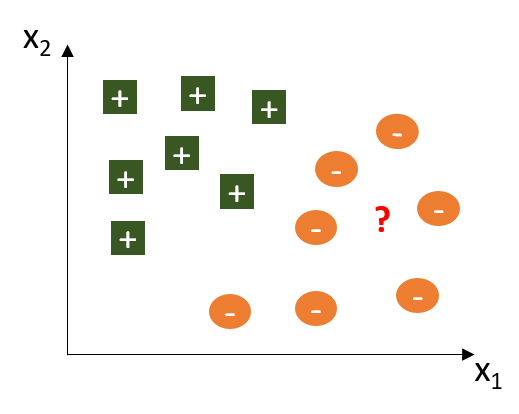
\includegraphics[width=0.7\textheight, clip]{images/example_hypothesis}\\
		\column{0.55\linewidth}
		\begin{itemize}
			\item How would you classify the test point ({\color{red}?}) ? 
			\item What drove you to make that choice? What is the assumption behind your choice?
		\end{itemize}
	\end{columns}
\centering\pause
 \textbf{Assumption:} Similar inputs have similar outputs
\end{frame}

\subsection{Formalization}
\begin{frame}{$k$ Nearest Neighbors: Formalization}
		\begin{columns}
		\column{0.6\textwidth}
		\textbf{Data Assumptions:}\\
		Similar $\boldx$ have similar $\smally$
		\pause
		\begin{equation*}
			\smally \in \mathbb{R} \text{ - regression}
		\end{equation*}
	\vspace{-0.6cm}
		\begin{equation*}
			\smally \in \mathcal{C} \text{ - classification}
		\end{equation*}
	
	\vspace{0.4cm}
	\pause
		\textbf{Definition of the $k$ nearest neighbors:}
		
		Given a test point $\unseenx$, let us denote $\knnset_\unseenx$ as its set of $k$ nearest neighbors. Formally: 
		
		%\vspace{-0.1cm}
		\column{0.4\textwidth}
		\begin{center}
			\onslide
			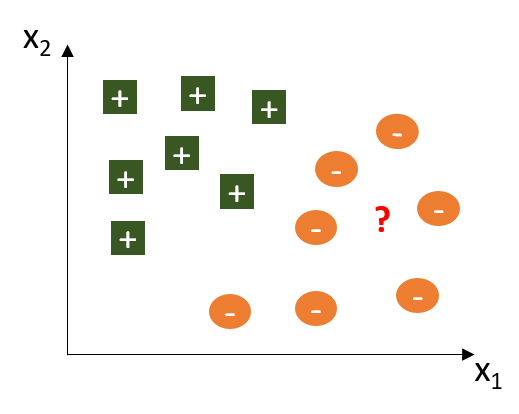
\includegraphics[width=\linewidth, clip]{images/example_hypothesis}
		\end{center}
	\end{columns}
\pause
\begin{align*}
	{\knnset_\unseenx} \subseteq \trainset \text{ .s.t. } &  |\knnset_\unseenx| = k  \\
	& \forall \, (\boldx', \smally') \in \trainset \setminus \knnset_\unseenx \,\, \text{dist}(\unseenx,\boldx') \geq \max_{(\boldx'', \smally'') \in \knnset_\unseenx} \text{dist}(\unseenx,\boldx'')
\end{align*}
	
%	\begin{itemize}
%		\item They use the observations in the training set $\trainset$ closest in input space to $\bigX$ to form $\predy$.
%		\pause
%		\item The K-nearest neighbor model fit is defined as follows:
%		\begin{equation}
%			\hypothesis(\unseenx) = \dfrac{1}{K}\sum_{\boldx_i \in \mathcal{N}_K(\unseenx)} \smally_i
%		\end{equation}
%		where:
%		\begin{itemize}
%			\item $\hypothesis$ - fitted function
%			\item $\unseenx$ - unseen data point
%			\item $\mathcal{N}_K(\unseenx)$ - the neighborhood of $\unseenx$ defined by the $K$ closest points $\boldx_i$ in the training sample
%		\end{itemize}
%		\pause
%		\item \textbf{Closest} implies a metric. We will assume (for now) the Eucledian distance
%		\pause
%		\item \alert{\textbf{In words:}} Find the $K$ observations with  $\boldx_i$ closest to $\unseenx$ and average their responses
		
%		\item 
%		\pause
%		\item It can be used for \textbf{classification} or \textbf{regression}
%		\item \textbf{Classification:} An unseen point $\boldx$ is classified by a majority vote of its k nearest neighbors (kNN)
%		\item \textbf{Regression:} The output $\predy$ is the average of the values of k nearest neighbors.
		 
%	\end{itemize}
	 		
\end{frame}

\begin{frame}{$k$ Nearest Neighbors: Hypothesis}
	\begin{columns}
		\column{0.6\textwidth}
		
		\pause
		\textbf{Regression: } The output is the average of the values of $k$ nearest neighbors 
					\begin{equation}
						\predy = \hypothesis(\unseenx) = \dfrac{1}{k}\sum_{(\boldx''_i, \smally''_i) \in \knnset_\unseenx} \smally''_i
					\end{equation}
		
		\pause
		\textbf{Classification:} An unseen point $\unseenx$ is classified by a majority vote of its $k$ nearest neighbors:
		\begin{equation}
			\predy = \hypothesis(\unseenx) = \text{mode}(\lbrace \smally''_i:(\boldx''_i, \smally''_i) \in \knnset_\unseenx \rbrace)
		\end{equation}
		
	
		\column{0.4\textwidth}
		\begin{center}
			\onslide
			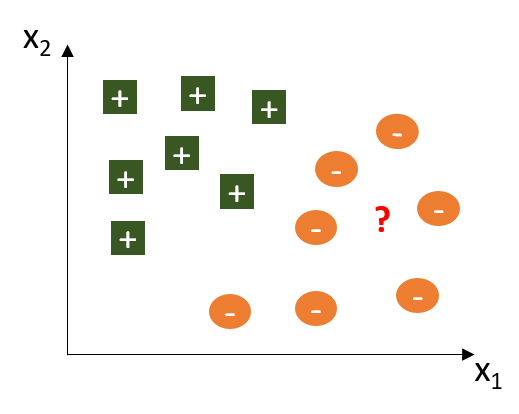
\includegraphics[width=\linewidth, clip]{images/example_hypothesis}
		\end{center}
	\end{columns}
	
\end{frame}

\subsection{Distance Metric}
\begin{frame}{Distance Metric}
	The definition of the set $\knnset_\unseenx$ is strongly dependent on the distance metric (dist) that is used. The better the chosen metric reflects the similarity among points the better the resulting model will be.
	
	\pause
	One of the most common metrics used is the Minkowski distance:
	\begin{equation}
		\text{dist}(\textbf{x},\textbf{z}) = \left( \sum_{j=1}^D |x_j -z_j|^p\right)^{1/p}
	\end{equation}

	\pause
	The main advantage of this metric is its generality. It contain many well-known distances as special cases.
	
	\alert{\textbf{Question:}} Can you identify what case is $p=2$? 
	
\end{frame}
	

\begin{frame}{\textit{Instance-Based Learning}}
	The k-NN algorithm differs from the "general" setup of supervised learning that we have seen so far. 
	
	\pause
	\vspace{0.4cm}
	It does not attempt to construct a general internal model, but simply stores instances of the training data.
	
	\pause
	\vspace{0.4cm}
	This type of approach is referred as 	\alert{\textbf{instance-based learning}} or \alert{\textbf{non-generalizing learning}}.
	
	\centering
	\vspace{0.4cm}
	\alert{\textbf{Question:}} Can you spot the differences?
	
\end{frame}

\section{Group Exercise}

%\subsection{Problem Statement}
%\begin{frame}[t]{Problem Statement}
%You are hired to implement the K-nearest neighbors for classification. Specifically, they request that you implement the two following functions:
%
%\vspace{1cm}
% \begin{columns}[t]
% 	 \column{0.45\linewidth}
% 	def train(\textit{*your params here*}):\\
% 	  \qquad  \textit{ ** Your pseudo code here **}
% 	\column{0.45\linewidth}
% 	def test(\textit{*your params here*}):\\
% 	 \qquad    \textit{** Your pseudo code here **}
% 	\end{columns}
%   
%\end{frame}

%\subsection{Requirements}
%\begin{frame}{Requirements}
%	As your client is completely new to machine learning, they have requested for you to answer to the following questions to help them get started with its use:
%	\begin{itemize}
%		\item What is the hypothesis class?
%		\item What are the assumptions about the data this hypothesis class makes?
%		\item What type of features can I use as input?
%		\item What is the output?
%		\item What value of $K$ I need to set?
%		\item What happens if $K=1$? $K=N$?
%		\item I want to check how good is my model. What would you recommend?
%	\end{itemize}
%\end{frame}
%%\begin{frame}{Setup: Training Data}
%%
%\pause
%
%	The data points $(\boldx_{i},\smally_{i})$ are drawn from an unknown probability distribution $\mathcal{P}(\bigX,\bigy)$.
%\end{frame}

\begin{frame}{Next steps}
	\begin{itemize}
		\item Split into groups
		\item Give your group a name (it will stay until the end of the course)
		\item Work on the solution together
		\item Come back to discuss it
	\end{itemize}	
\end{frame}	


	
\begin{frame}[t,standout]
	\Large
	Wrap-Up
\end{frame}

\begin{frame}{Summary: Notation}
	
	\begin{table}
		\begin{tabular}{|l | l | }
			\hline
			Symbol & Reads as \\
			\hline \hline
			$\bigX$ & Input variable $(\mathbb{R}^D)$ \\ 
			$\boldx_i$ & $i^{th}$ feature vector.  Observed value of $\bigX$.  \\
			$\mathbf{\bigx}=(\boldx_1,\boldx_2, \ldots, \boldx_N)^T$ & Matrix of $N$ input $D-$dimensional vectors $\boldx_i$\\
			$\smallx_{j}$ & $j^{th}$ element of the $i^{th}$ input vector $\boldx_i$, i.e. $\smallx_i^j$ \\ 
			$\bigy$ & Output variable  $(\mathcal{C})$\\ 
			$\smally_i$ & $i^{th}$ output label\\ 
			$\boldy=(\smally_1, \ldots, \smally_N)^T$ & Observed vector of outputs $\smally_i$\\
			$\unseenx$ & Test point (unseen data) \\
			$\predy$ & Prediction for $\unseenx$ \\
			\hline
		\end{tabular}
		\caption{Different notation for the input and output variables}
	\end{table}

\end{frame}

\begin{frame}{Further Reading and Useful Material}
	
	\begin{table}
		\begin{tabular}{|l | l | }
			\hline
			\multicolumn{1}{|c|}{\textbf{Source}} & \multicolumn{1}{c|}{\textbf{Notes}} \\
			\hline
			The Elements of Statistical Learning &	Ch. 2 \\
			\hline
		\end{tabular}
	\end{table}
	
	
\end{frame}

\end{document}
